%% ==============================
\chapter{Implementation}
\label{sec:implementation}
%% ==============================
The multi-floor navigation is implemented in Python 3.9 and later integrated into \gls{ros_2} Foxy. It is designed to be modular and can be easily integrated into the existing \gls{nav_2} stack. The planner is also designed to be scalable and can be used in environments of varying size and complexity. The behavior tree library BehaviorTree.CPP \cite{auryn_robotics_behaviortreecpp_2023} is used to coordinate all subtasks. Individual BT actions are programmed in C++ and can easily be used to interact with ROS 2 nodes. The hierarchical planner is implemented in a separate ROS 2 node completely written in Python. The most used libraries are NetworkX for graph building and planning, OpenCV for gridmap handling and image segmentation, and Shapely for collision checking during roadmap generation and path planning. All of these libraries are efficiently implemented and use C libraries under the hood to speed up the computation. The code produced in this work is mainly written in Python, as it is faster to prototype and well-documented libraries for graph handling exist. This work does not claim to have a very efficient implementation or the best performance, it is only meant as a proof of concept.

%% ==============================
\section{Hierarchy Creation}
\label{sec:hierarchy_creation}
%% ==============================
The input for the hierarchy creation is the raw occupancy gridmap from the robot's SLAMing process. The same benchmark map used for the algorithm from \cite{ryu_hierarchical_2020} is used for evaluation and better comparison. For better readability, the image of this raw occupancy gridmap from Chapter \ref{sec:benchmarks} is shown again here in Figure \ref{fig:freiburg_benchmark_2}.

\begin{figure}[h]
    \centering
    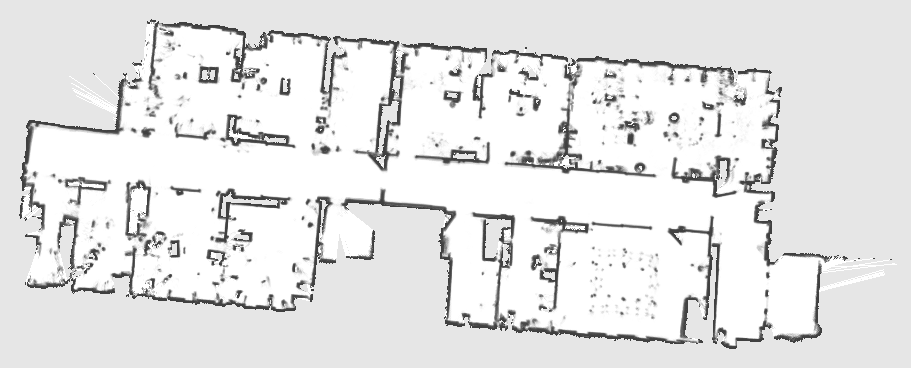
\includegraphics[width=0.75\textwidth]{figures/30_methods/freiburg_benchmark.png}
    \caption[The benchmark environment for hierarchy creation and straight path planning (intentional repetition)]{The benchmark environment for hierarchy creation and straight path planning recorded in the University of Freiburg (Source: \cite{cyrill_stachniss_robotics_2015})(intentional repetition)}
    \label{fig:freiburg_benchmark_2}
\end{figure}

This gridmap is built with the mobile robot's laser scanners, starting from the current pose at the time the mapping is started. This starting pose is often not aligned with the surrounding walls, resulting in an apparent angle between the walls and the coordinate frame of the gridmap. This is not a problem for localization or path planning, but makes it difficult to plan straight paths parallel to the walls. To solve this problem, a rotation detection and outlier reduction algorithm is used.

\begin{figure}[h]
    \centering
    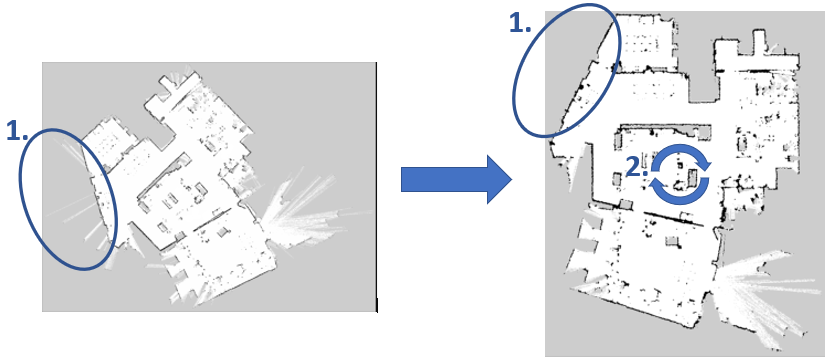
\includegraphics[width=0.75\textwidth]{figures/50_implementation/model_preprocessing_goal.png}
    \caption[Map preprocessing with rotation and outlier detection]{Map preprocessing with rotation and outlier detection. Original map on the left with outliers caused by transparent windows (1.). Resulting map on the right, outliers removed (1.) and rotation aligned with wall directions (2.) (Source: Tim Albert)}
    \label{fig:map_preprocessing}
\end{figure}

Figure \ref{fig:map_preprocessing} shows the result of the preprocessing algorithm. The algorithm first performs dilation and detects connected components. Based on their size, these components are classified as outliers and the corresponding walls and white trails in 1. are removed. Then the Probabilistic Hough Transform \cite{matas_robust_2000} is used to detect straight lines representing the walls of the rooms. Finally, the main orientation is chosen based on the majority of wall lines going in the same direction. To consider a single wall of a room and its perpendicular neighbor, the detected lines are clustered with \gls{dbscan} algorithm \cite{ester_density-based_1996}. After obtaining the major rotation angle of the walls, the entire map is rotated to align with the coordinate frame of the gridmap. Since this was developed and tested in an independent project, it is outside the scope of this work.

The resulting map is now rotated parallel to the walls and outliers are removed. However, there are still some artifacts in the map that obscure the true shape of the room. For best results, some manual cleaning is still required. Most of these artifacts are dynamic obstacles that were at these positions during the mapping process, but could have moved to another location by now. In order not to depend on this current snapshot of the environment, the real shape of the room is estimated. The obstacles are later taken into account during the actual driving process. The task of the controller is to avoid these obstacles and provide a path around them. If this is not possible within the limits of the controller, a replan is triggered. The resulting cleaned map is then binarized with a threshold and can be seen in Figure \ref{fig:map_cleaned}.

\begin{figure}[h]
    \centering\captionsetup{justification=centering}
    
\includegraphics[width=0.75\textwidth]{figures/50_implementation/ryu.png}
    \caption[Binary map after rotation and manual cleaning]{Binary map after rotation and manual cleaning}
    \label{fig:map_cleaned}
\end{figure}

The segmentation of this map into individual rooms and corridors is now done with the marker-controlled watershed algorithm \cite{parvati_image_2009}. The gridmap is converted to a numpy matrix and processed with OpenCV. OpenCV provides implementations of common image processing operations in Python that can be used to create the watershed representation. The process begins by creating markers to enhance the normal watershed algorithm. Without predefined markers, the watershed results in over-segmentation. To do this, a distance transform is performed on the image from Figure \ref{fig:map_cleaned}. This creates a mapping of each white pixel's distance to the nearest black pixel. This can be interpreted as the obstacle clearance of that position and corresponds to the safety cost mask of Seder et al. \cite{seder_hierarchical_2011}. By thresholding this distance map to a reasonable distance value \(d\), the resulting binary image shows in white all pixels that have a distance greater than or equal to \(d\), as seen in Figure \ref{fig:distance_transform}. This represents the areas where most likely rooms are located. 

\begin{figure}[h]
    \captionsetup[subfigure]{justification=centering}
    \centering
    \begin{subfigure}{.5\textwidth}
      \centering
      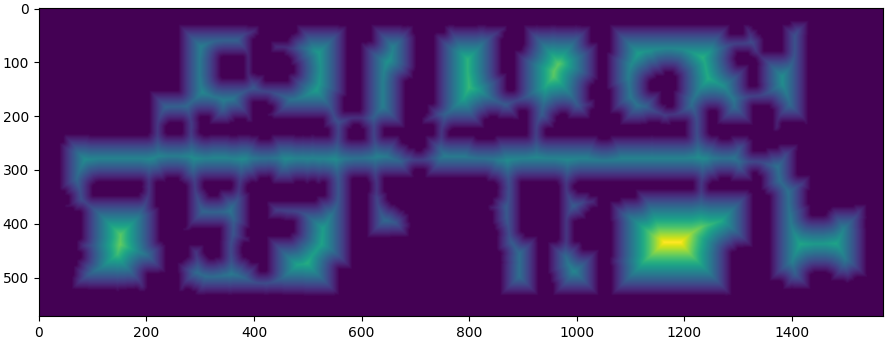
\includegraphics[width=\textwidth]{figures/50_implementation/ryu_distance_transform.png}
      \caption{Distance transform}
    \end{subfigure}%
    \begin{subfigure}{.5\textwidth}
      \centering
      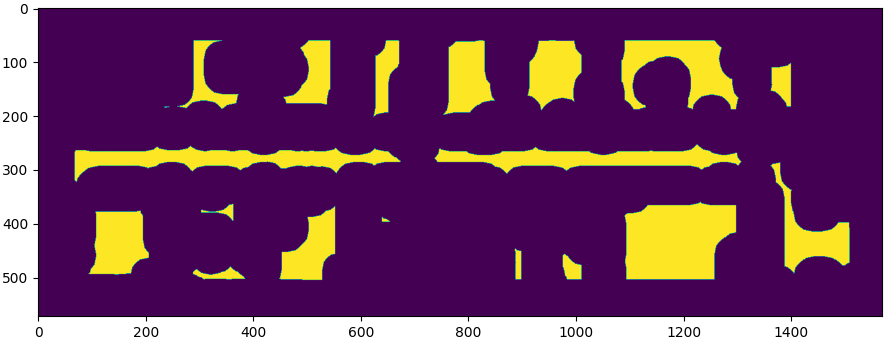
\includegraphics[width=\textwidth]{figures/50_implementation/ryu_markers.png}
      \caption{Markers as binary threshold of (a)}
    \end{subfigure}
    \caption[Distance transform and resulting markers]{Distance transform (a) and resulting markers (b) as initial information for the watershed algorithm.}
    \label{fig:distance_transform}
\end{figure}

To get the number, outlines, and areas of each segment, the OpenCV function for detecting connected components is called and returns a list of each area. With this list as input, the watershed is then marker-controlled and provides a good segmentation of the entire floor into separate rooms, as seen in Figure \ref{fig:watershed}.

\begin{figure}[h]
    \centering\captionsetup{justification=centering}
    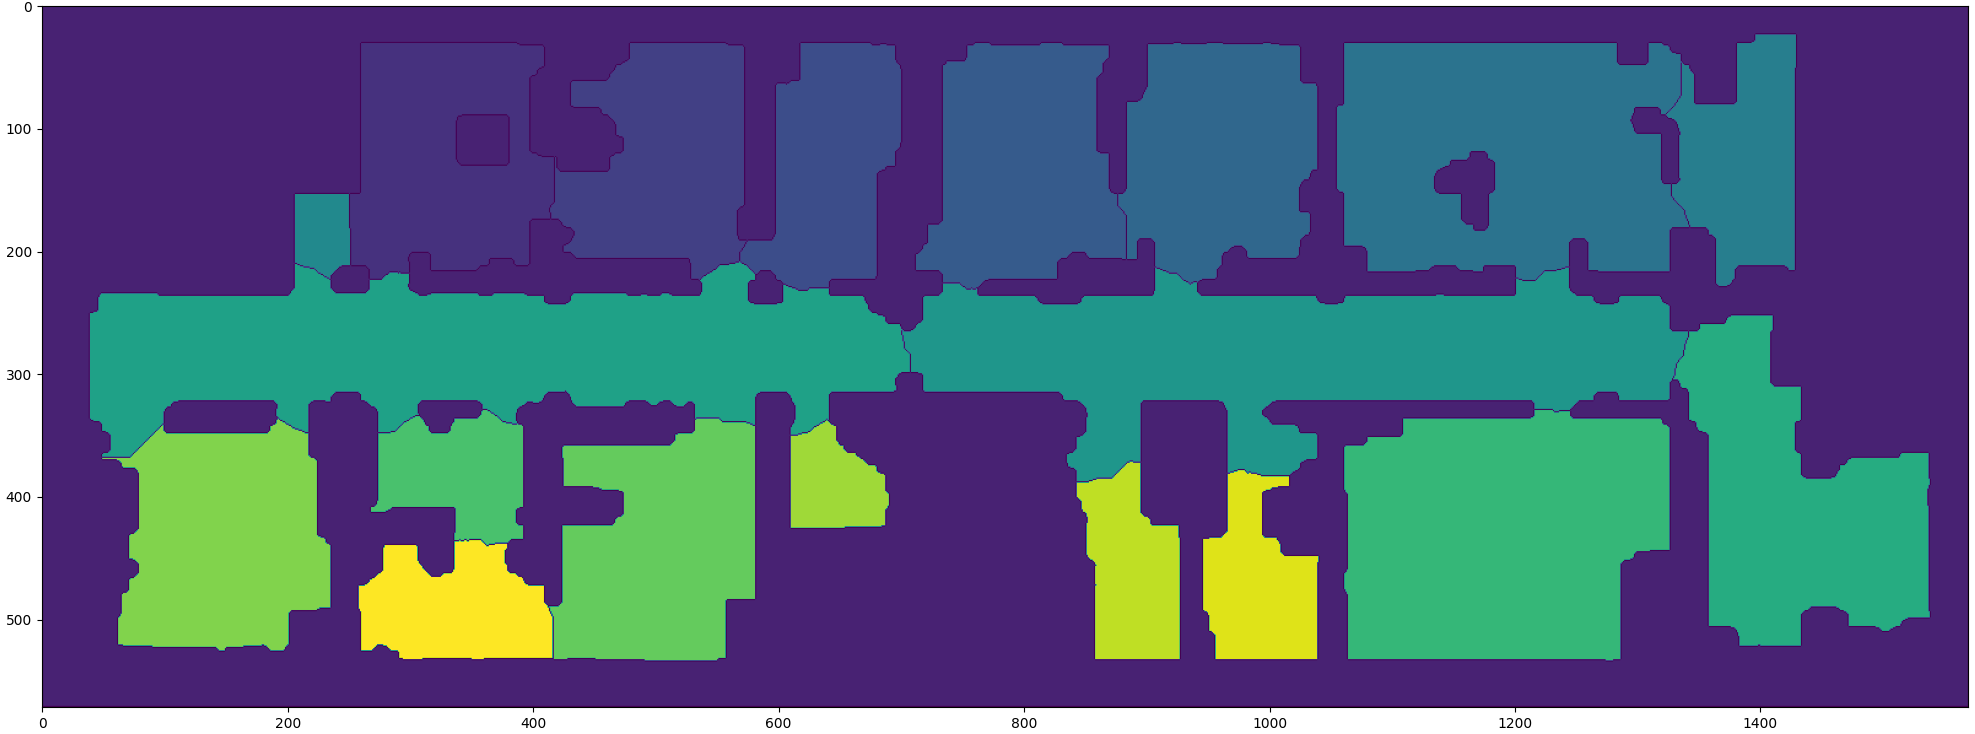
\includegraphics[width=0.75\textwidth]{figures/50_implementation/ryu_watershed.png}
    \caption[Marker-controlled watershed of the benchmark map]{Marker-controlled watershed of the benchmark map}
    \label{fig:watershed}
\end{figure}

This room segmentation provides the area for each room. To create a hierarchical graph from this, the doors between them are important to create a hierarchical connection in the floor graph. The algorithm used in this work is based on the junction node extraction algorithm proposed by Ryu \cite{ryu_hierarchical_2020}. The basis for this algorithm is the result of the watershed segmentation of Figure \ref{fig:watershed}. First, an adjacency matrix of the rooms is created. If rooms are directly connected to each other with only a border created by the watershed between them, they have a real-world connection. This connection and all pixels on this border are stored. The distance transform from Figure \ref{fig:distance_transform} (a) is then used to look up the pixel with the maximum distance to the walls from this list of pixels on the border. Repeating this step for all connections in the adjacency matrix results in the bridge points with the maximum distance to the wall. 

\begin{figure}[h]
    \captionsetup[subfigure]{justification=centering}
    \centering
    \begin{subfigure}{.65\textwidth}
      \centering
      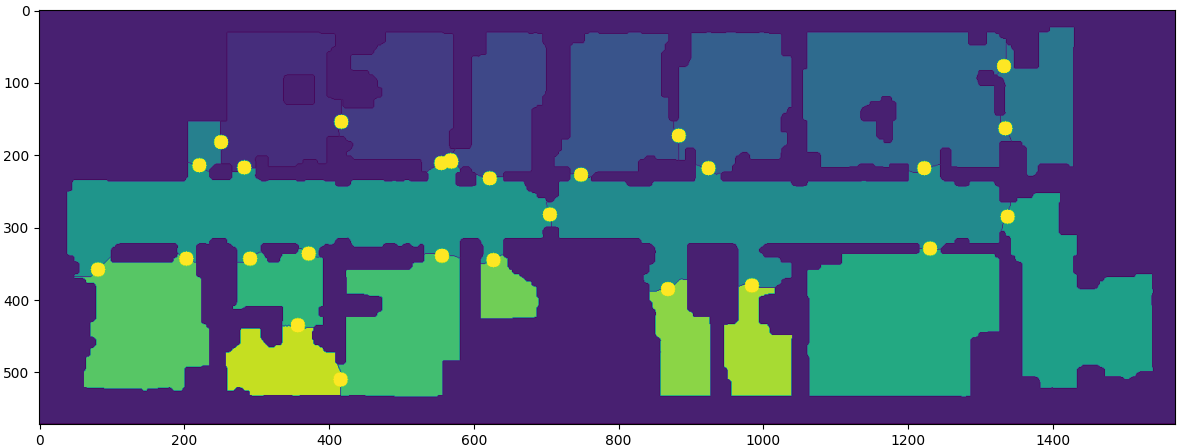
\includegraphics[width=\textwidth]{figures/50_implementation/ryu_bridge_nodes.png}
      \caption{Watershed result with detected bridge points}
    \end{subfigure}%
    \begin{subfigure}{.25\textwidth}
      \centering
      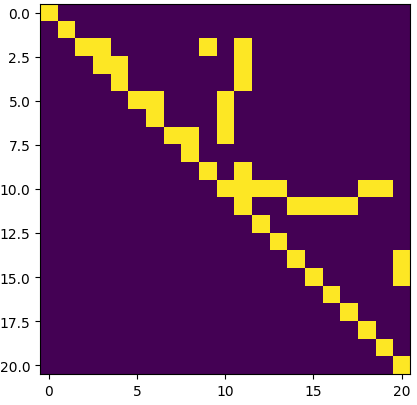
\includegraphics[width=\textwidth]{figures/50_implementation/ryu_adjacency_matrix.png}
      \caption{Adjacency matrix}
    \end{subfigure}
    \caption[The result of the bridge point detection algorithm]{The result of the bridge point detection algorithm. Bridge points overlaid on the segmented map (a). The adjacency matrix of the rooms (b), where all rooms are drawn on the axis and a yellow pixel represents a connection between them. Rooms always have pixels connecting them to themselves (diagonal line).}
    \label{fig:bridge_nodes}
\end{figure}

The floor segmented into rooms and their connections expressed as bridge points can now be represented as a graph. Each room becomes a node in the floor graph. Each bridge point represents a door and becomes an edge in the graph. The corresponding graph can be seen in Figure \ref{fig:ryu_graph}. Note that this is inverted on the y-axis because all previous map images were taken from OpenCV, which by default has its origin for images in the top left corner. In comparison, the graphs are taken from NetworkX, which has its origin in the bottom left corner. 

\begin{figure}[h]
    \centering
    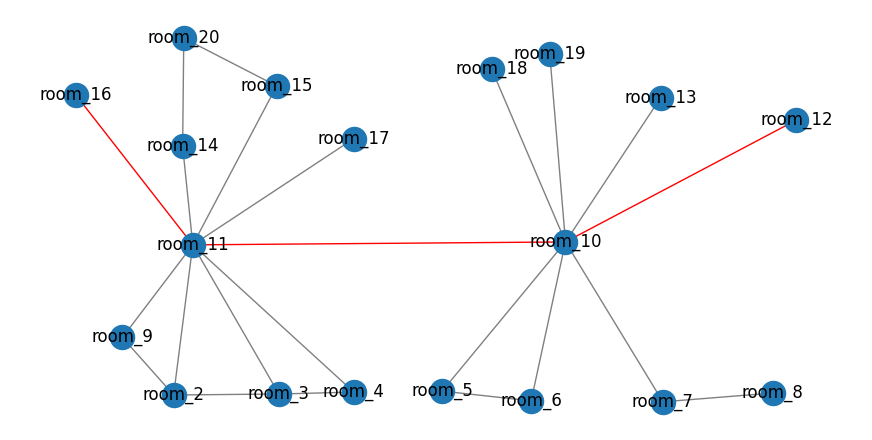
\includegraphics[width=0.7\textwidth]{figures/50_implementation/ryu_floor_graph.png}
    \caption[Graph representation of the benchmark map]{Graph representation of the benchmark map. Nodes are rooms and edges represent doors between them. In red is an example path from room 16 to room 12.}
    \label{fig:ryu_graph}
\end{figure}

To create an H-Graph for this benchmark, each room node must itself contain a graph. These subgraphs are then the lowest hierarchical level and represent the roadmap of each room. Each roadmap consists of collision-free paths on the corresponding room gridmap. The straight path planner ILIR is used to create these roadmaps.

%% ==============================
\section{Roadmap Generation}
\label{sec:roadmap_generation}
%% ==============================
The first step in path planning is to convert the environment into a Shapely object. This has the advantage that basic shapes like lines, rectangles and polygons are available, collision checks between these shapes are already efficiently implemented with a C library, and the precision is higher than with pixel-based images. The images from OpenCV represent the environment in discrete pixels, which is helpful because the gridmap recorded by the laser scanners has exactly this resolution. However, for collision checking and creating paths as lines, it is important to model these shapes accurately. Lines should be one-dimensional shapes that have no area. In comparison, a line in a numpy matrix as used by OpenCV is represented by a series of pixels, each with a certain width and height. This leads to unexpected behavior and incorrect results. The converted shapely environment can be seen in Figure \ref{fig:ryu_shapely}

\begin{figure}[h]
    \centering
    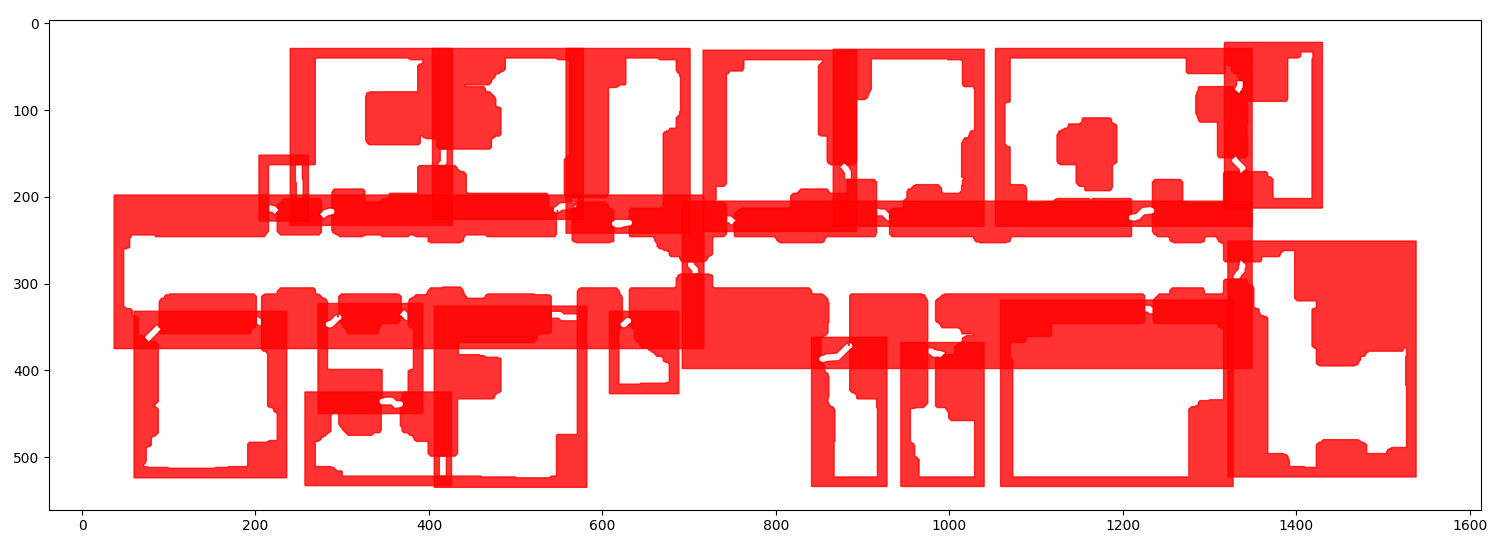
\includegraphics[width=0.75\textwidth]{figures/50_implementation/ruy_shapely.png}
    \caption[Shapely representation of the benchmark map]{Shapely representation of the benchmark map. Each room has its own environment and is surrounded by red obstacles. All room environments are drawn in a single image for visualization, resulting in overlapping red obstacles.}
    \label{fig:ryu_shapely}
\end{figure}

In each room, the largest interior rectangles are searched for in an iterative process and combined to form a polygon. The algorithm for finding the largest interior rectangle (LIR) is by Marzeh et. al \cite{marzeh_algorithm_2019} and the Python implementation used is by Weber \cite{weber_largest_2023}. The proposed Iterative Largest Interior Rectangle (ILIR) algorithm extends these ideas by repeatedly searching for the largest rectangle. The Algorithm \ref{lst:pseudo_code_ilir} shows the pseudocode of the ILIR straight path planner. In each room the LIR algorithm is executed (line 14) and later the found rectangle is subtracted from the original area and the same process is repeated with the remaining area (line 21). This not only produces the largest rectangle, but also a polygon that is aligned with the axis of the coordinate frame. Simply finding the largest interior polygon would not be useful, because at high resolution this would only approximate the original shape. Also, the edges of this polygon would not be parallel to the walls of the room, which is an important requirement for the proposed algorithm. Additionally, for each rectangle it is decided whether the shape belongs to a corridor or a room based on predefined parameters (line 16). For a corridor, the rectangle is collapsed to a straight line to provide a better path for the robot. This process is repeated for each room until the area of the largest remaining contour is below a predefined threshold (line 10). All paths are stored in a list, which corresponds to the roadmap. Finally, the rectangles found are merged into a polygon (line 24) and the bridge points to other rooms are connected to it (line 26).

\lstset{language=C++, mathescape=true, caption={Pseudocode of the ILIR Straight Path Planner}, label={lst:pseudo_code_ilir}, morekeywords={from, to, is, Input, Output, each, in, end, do, then, Algorithm}}
\begin{lstlisting}[float=h]
Algorithm: Iterative Largest Interior Rectangle (ILIR)
Input: gridmap, parameter
Output: roadmap

room_list $\gets$ markerControlledWatershed(gridmap)

bridge_points $\gets$ extractBridgePoints(room_list)

for each room in room_list do:

    while largest_contour.area > parameter.min_area do:
    
        largest_contour $\gets$ maxContourByArea(room)
            
        largest_rectangle $\gets$ largestInteriorRectangle(largest_contour)

        if isCorridor(largest_rectangle) then:
            room.roadmap.add(centerLine(largest_rectangle))
        else
            room.roadmap.add(largest_rectangle)

        room $\gets$ (room - largest_rectangle)
    end

    room.roadmap $\gets$ mergeRectangles(room.roadmap)
    
    room.roadmap.add(connectBridgePoints(bridge_points))
end
\end{lstlisting}

In Figure \ref{fig:ilir_room_roadmap}, the ILIR algorithm is applied to room 2 of the benchmark map. The red Shapely environment represents the \(C\) space for the path planning problem. The free area from (a) is converted to \(C\) space and a safety margin is applied to the walls and obstacles using a dilation operation.  Therefore, obstacles in the \(C\) space look larger than they are in the real world. This safety margin depends on the size of the robot and additional safety considerations. This allows to treat the robot as a point in \(C\) space and still ensure a collision free path. 
\begin{figure}[h]
    \captionsetup[subfigure]{justification=centering}
    \centering
    \begin{subfigure}{.235\textwidth}
      \centering
      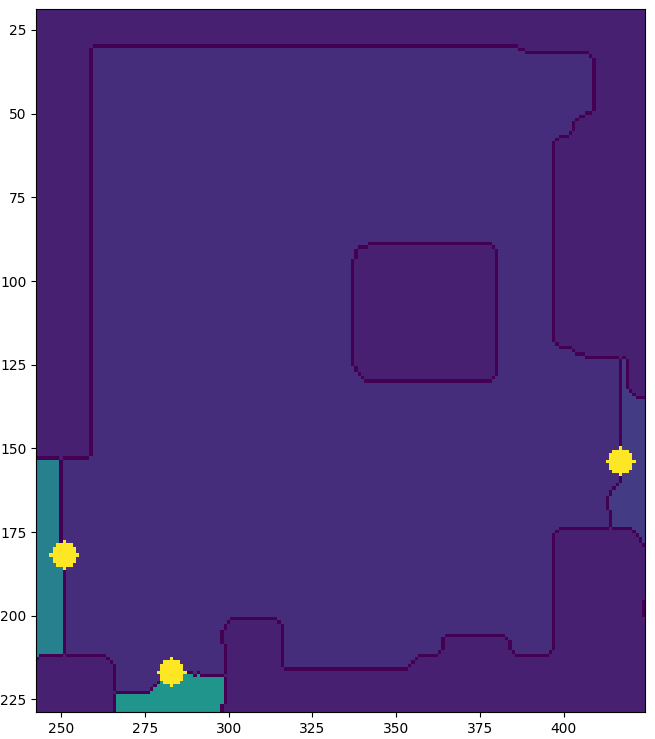
\includegraphics[width=\textwidth]{figures/50_implementation/ryu_room2_clean.png}
      \caption{Room after segmentation}
    \end{subfigure}%
    \begin{subfigure}{.25\textwidth}
      \centering
      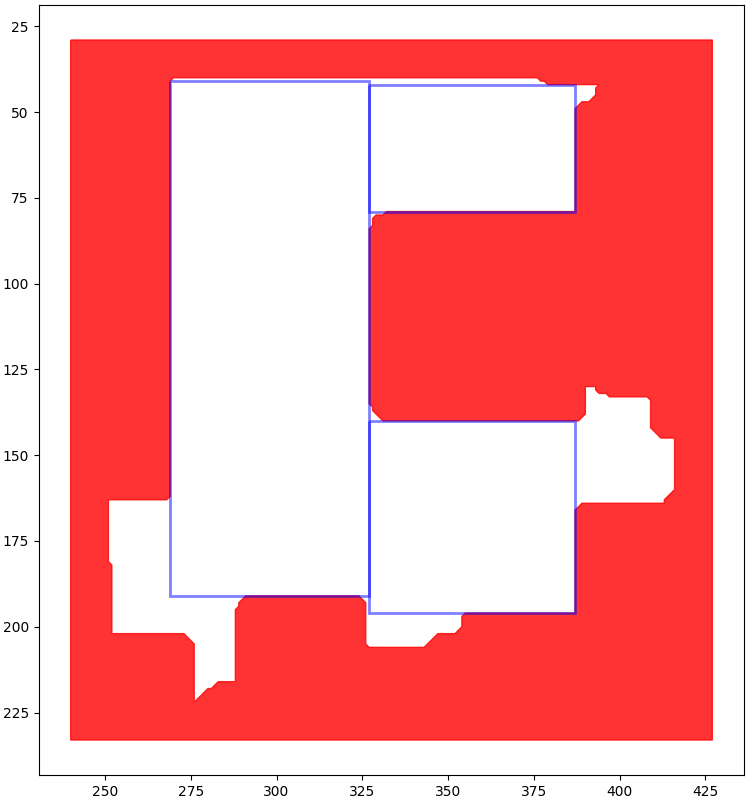
\includegraphics[width=\textwidth]{figures/50_implementation/ryu_room2_rectangles.png}
      \caption{Largest interior rectangles}
    \end{subfigure}%
    \begin{subfigure}{.25\textwidth}
      \centering
      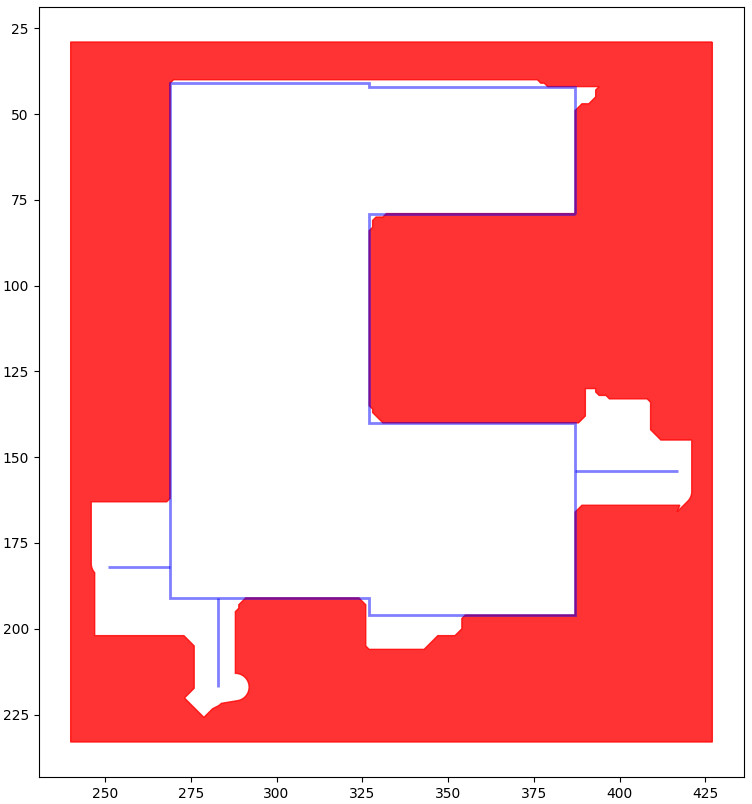
\includegraphics[width=\textwidth]{figures/50_implementation/ryu_room2_roadmap.png}
      \caption{Roadmap as produced by ILIR}
    \end{subfigure}%
    \begin{subfigure}{.25\textwidth}
      \centering
      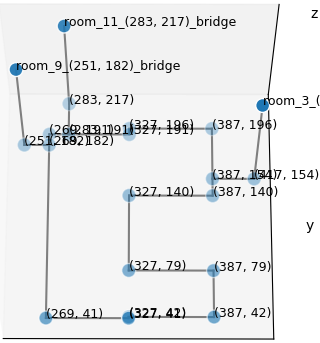
\includegraphics[width=\textwidth]{figures/50_implementation/ryu_room2_roadmap_graph.png}
      \caption{Roadmap converted to a graph}
    \end{subfigure}
    \caption[Application of the ILIR straight path planner on room 2 from the benchmark map]{Application of the ILIR straight path planner on room 2 from the benchmark map. The red obstacles are enlarged by the robot's radius to ensure collision-free paths. Note that the y-axis of the graph is inverted compared to the other images.}
    \label{fig:ilir_room_roadmap}
\end{figure}
As the last step of the ILIR algorithm, the doors of neighboring rooms are connected to the merged rectangles. In Figure \ref{fig:ilir_room_roadmap} (a), three doors to other rooms can be seen as yellow dots. These are then connected to the polygon to form the resulting roadmap in (c). These connections are created by first checking the straight line with the shortest distance between the door and the roadmap. If this line collides, an A* search is performed to find the shortest possible connections. The resulting A* path is then smoothed and converted into a series of straight lines that are added to the roadmap. For actual path planning in the real world, the robot can be at any valid position in the room and must first find a collision-free path to the roadmap before it can follow the roadmap to the door of the next room or an elevator to the next floor. This linking of start and end positions, which may or may not be on the roadmap, is done by the same process and can be seen in the next chapter in Algorithm \ref{lst:pseudo_code_ilir}. To make this roadmap searchable in an H-Graph, it is converted to nodes and edges in the corresponding room graph (d). The connections in the z-axis represent the hierarchical connections to another graph. They have no path cost and are therefore not considered in the total distance of the path. By repeatedly applying the ILIR algorithm to each room in the previously segmented gridmap, the H1 and H2 levels of the H-Graph can be automatically generated. Figure \ref{fig:ryu_roadmap} shows a visualization of all roadmaps of each room combined and overlaid on the watershed image.

\begin{figure}[h]
    \centering
    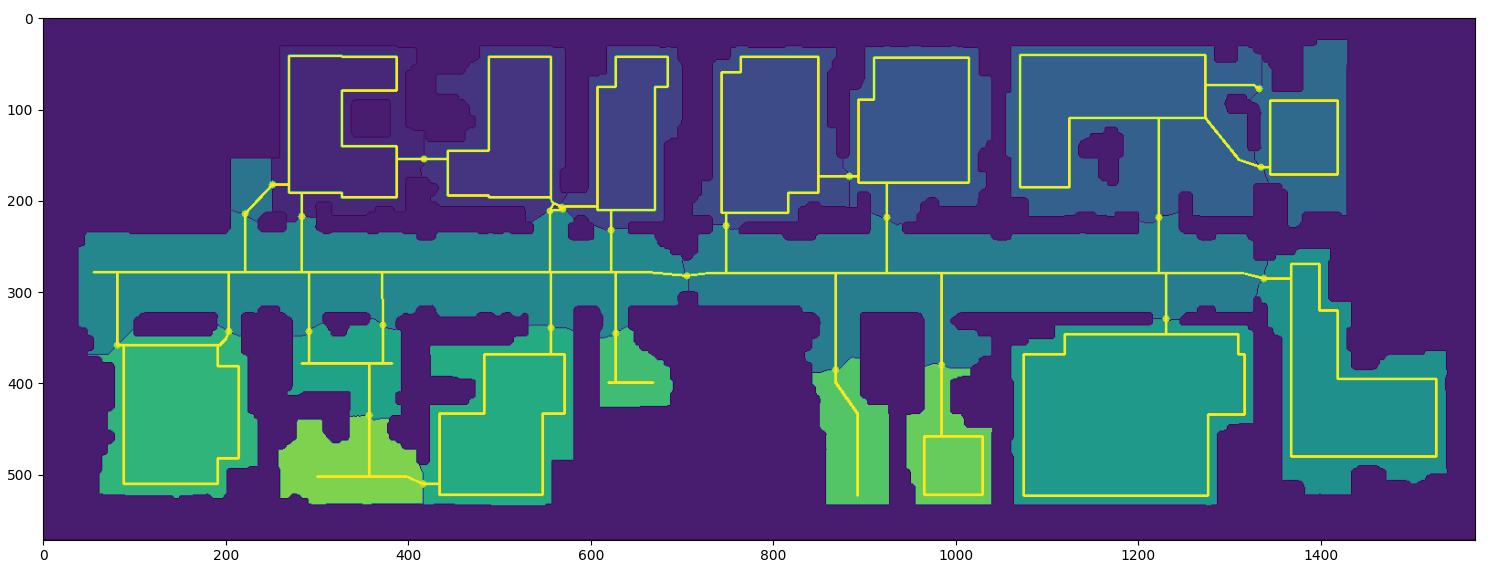
\includegraphics[width=0.75\textwidth]{figures/50_implementation/ryu_roadmap.png}
    \caption[Roadmap of the entire floor combined]{Roadmap of the entire floor combined and overlaid on the result of the Watershed algorithm. Note that the paths in the corridors are collapsed to a single line in the center.}
    \label{fig:ryu_roadmap}
\end{figure}

The ILIR algorithm is capable of finding a solution if a solution exists. This is ensured by the A* planner, which is both complete and optimal. Thus, ILIR is also complete. However, although the A* is used for bridge point connections, the rest of the generated roadmap cannot guarantee the shortest path. Thus, the ILIR algorithm produces a path that is not optimal in terms of path length.

%% ==============================
\section{Hierarchical Planning}
\label{sec:impl_hierarchical_planning}
%% ==============================
An overview of the different components for hierarchical path planning was given in Chapter \ref{sec:hierarchical_planning}. Figure \ref{fig:h_graph_uml} shows a more detailed UML diagram of the H-Graph implementation. The Coordinator and the Environment Model work as described in the concept chapter. The focus here is on the specific implementation of the H-Graph and its recursive hierarchical planning method.

\begin{figure}[h]
    \centering
    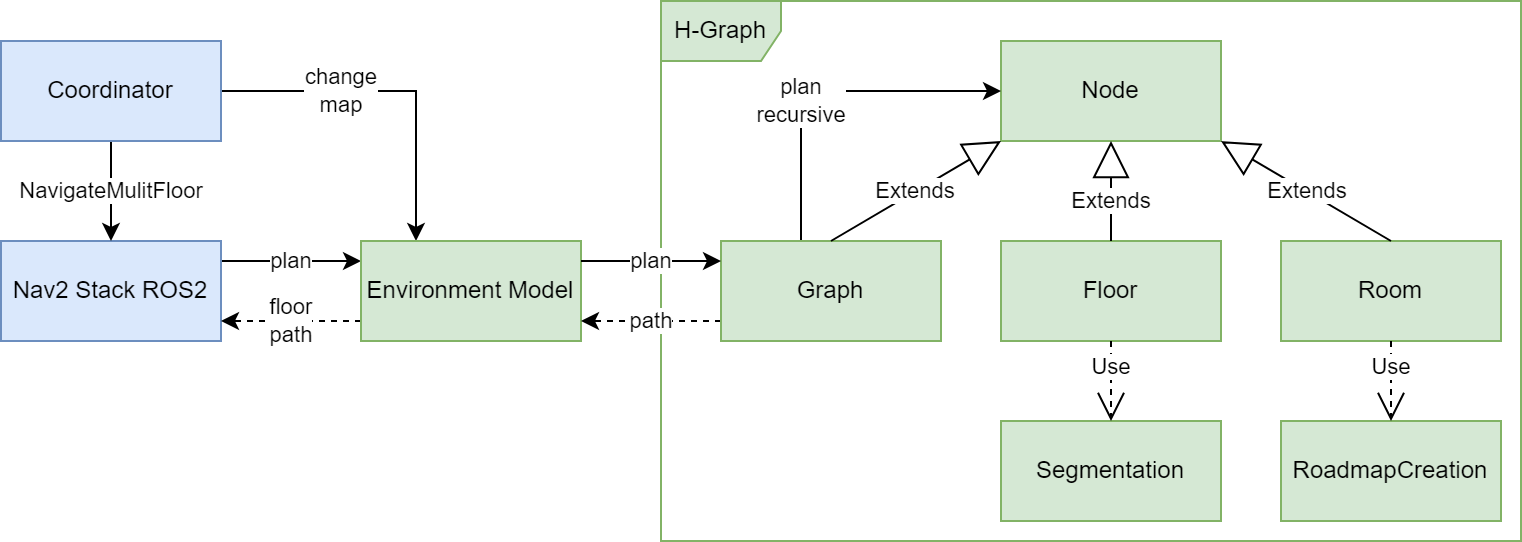
\includegraphics[width=\textwidth]{figures/50_implementation/h_graph_uml.png}
    \caption[UML diagram of the H-Graph implementation]{UML diagram of the H-Graph implementation. Blue components were taken from the community, green components were developed in this work.}
    \label{fig:h_graph_uml}
\end{figure}

The base class for any component in the H-Graph is the Node. This class implements all the basic functions needed to operate as a hierarchically structured graph. This includes a private variable that holds the corresponding subgraph of the next lower hierarchy. Each node of the subgraph is again of type Node. The public methods of Node are for adding and retrieving nodes and connections to the subgraph, as well as a function for planning with the Dijkstra algorithm in the subgraph and another function for planning recursively between arbitrary nodes in the H-Graph. This function first plans the path in the subgraph and then passes the planning process to each node in that path on the next lower hierarchy level. Details of the implementation of this recursive algorithm are given in Algorithm \ref{lst:pseudo_code_recursive}. To start this recursive planning process, it must be initialized with some values such as the unique start and goal positions in the hierarchy and the initial path on the subgraph. This is done by the Graph class, which inherits from Node and represents a specialization of its functionality. This Graph node usually exists only once because it represents the root of the H-graph, initializes recursive functions, and provides some visualization functions. The other specializations of Node are the Floor and Room classes. These are important for initially building the H-graph from the gridmap data. The Floor class performs the segmentation process and creates the correct number of Room nodes in its subgraph. Each Room triggers the creation of the roadmap in its corresponding area from the segmented gridmap. Since these specializations all inherit from the base Node class, they use the same recursive hierarchical planning process. A finite number of hierarchy levels can be created in an H-Graph. The planning process still works the same and will find a solution if possible. Because a building or a campus does not have any special functions that need to be separated from normal nodes, it is not implemented as a separate class. These nodes are just inserted into the H-Graph as plain node objects, just like bridge nodes, which are only necessary for the planning process.

\lstset{language=C++, mathescape=true, caption={Pseudocode of Hierarchical Path Planning}, label={lst:pseudo_code_planning}, morekeywords={from, to, is, Input, Output, each, in, end, then, Algorithm}}
\begin{lstlisting}[float=h]
Algorithm: Hierarchical Path Planning
Input: start_hierarchy, goal_hierarchy, h_graph
Output: path

for hierarchy in [start_hierarchy, goal_hierarchy] do:

    room, pos $\gets$ getHierarchyH2(hierarchy)
    
    if pos not in room.roadmap then:
    
        if noCollision(straightLine(pos, room.roadmap)) then:
        
            path $\gets$ straightLine(pos, room.roadmap)
            
            room.roadmap.add(path)
        else:
            path $\gets$ A*Planner.plan(pos, room.roadmap)
            
            room.roadmap.add(path)
end

path $\gets$ RecursiveHierarchicalPlanner.plan(
            start_hierarchy, goal_hierarchy, h_graph)

\end{lstlisting}

The first step of the whole navigation process is the trigger from the Coordinator to the \gls{nav_2} stack, which passes it to the responsible planner plugin. This is the custom Hierarchical Planner, which then sends a ROS 2 action goal to the environment node. The interfaces of the process up to this point will be presented later in the next Chapter \ref{sec:multi_floor_behavior_trees}. At this point, the ROS 2 action server of the Environment Model node starts the hierarchical planning. This process is shown in Algorithm \ref{lst:pseudo_code_planning}. The path planning starts by checking if the given start and goal positions are already in the roadmap of the corresponding room (line 9). If they are not in the roadmap, they have to be connected with a path. For this, the straight line between the position and the nearest point in the roadmap is checked for collisions (line 11). If this line is free, the connection is added to the roadmap and the position is now part of the subgraph and can be searched by the following planning process. If the straight connection is not possible because of an obstacle, the shortest path around the obstacle is searched with the A* algorithm (line 17). This is guaranteed to find a solution if it is possible. After both the start and goal locations have been added to the roadmap, it is now possible to find the solution by searching the H-Graph. Since these locations can be on very different parts of the environment and therefore on different branches of the hierarchical structure, the proposed recursive hierarchical planner is needed to search through each hierarchy of the H-Graph. This process is described later in the Algorithm \ref{lst:pseudo_code_recursive}.

\lstset{language=python, mathescape=true, caption={Unique H-Graph positions and path representation}, label={lst:pseudo_code_datastructure}, morekeywords={from, to, is, input, output, each, in, end}}
\begin{lstlisting}[float=h]
# general description of a unique position:
$p = \{p_{Hn}, p_{Hn-1}, ..., p_{H1}\}$

# specific unique position with 4 hierarchies in Python:
p_hierarchy = ["Building F", "Floor 2", "Room 2", (50,210)]

# specific example path with 4 hierarchies in Python:
path = {
    "Building F": {
        "Floor 3": {
            "Meeting Room": {...},
            "Corridor": {...},
            "Elevator": {...},
            "Floor 2_Elevator_bridge": {}
        },
        "Floor 2": {
            "Floor 3_Elevator_bridge": {},
            "Elevator": {...},
            "Corridor": {...},
            "Terrace2": {...},
            "Terrace_Floor 1_Ring F_bridge": {}
        },
        "Terrace_Floor 1_bridge": {}
    },
    "Terrace": {
        "Building F_Floor 2_bridge": {},
        "Floor 1": {
            "Building F_Floor 2_Terrace2_bridge": {},
            "Ring F": {...}
        }
    }
}
\end{lstlisting}

But first, the datastructure of such a unique hierarchical position and the path through the H-Graph must be explained. In Algorithm \ref{lst:pseudo_code_datastructure} the general description of a unique position in the H-Graph can be seen (line 2). The position consists of the specific nodes of each subgraph for all hierarchies from top (\(Hn\)) to bottom (\(H1\)). As an example, the unique description of a position in a 4-level H-Graph is shown in line 5. The highest hierarchy level is buildings and the lowest is the specific position on the gridmap. Since the node in for NetworkX can have any hashable value, a tuple is used for the position. The datastructure of a complete path through the H-Graph is shown in lines 8-32. For the sake of clarity, the lowest hierarchy (\(H1\)), the positions on the gridmap, is omitted, since the general structure is clear even with the top three levels. The path is represented as a nested dictionary, each entry in the dictionary has a key, the node in the path of the current hierarchy level, and a value, which is another dictionary containing the path on the subgraph of the key node. Note that bridge nodes do not have a subgraph of their own as they only connect the hierarchies. As of Python 3.7, dictionaries are guaranteed to keep insertion order. This allows it to store the nodes in the correct order as they appear on the actual path. 

\lstset{language=C++, mathescape=true, caption={Pseudocode of the recursive planning function}, label={lst:pseudo_code_recursive}, morekeywords={from, to, is, Input, Output, each, in, end, then, enumerator, Algorithm, with}}
\begin{lstlisting}[float=h]
Algorithm: recursiveHierarchicalPlanning
Input: child_path, start_hierarchy, goal_hierarchy, hierarchy_level
Output: path

for node in child_path with enumerator i do:

    if isLeaf(node) or isBridge(node) then:
        path[node] $\gets$ {}
        continue

    if node is child_path[-1] then:
        child_graph_goal $\gets$ goal_hierarchy[hierarchy_level+1]
    else:
        child_graph_goal $\gets$ getBridgeTo(node, child_path[i+1])
        
    if node is child_path[0] then:
        child_graph_start $\gets$ start_hierarchy[hierarchy_level+1]
    else:
        child_graph_start $\gets$ getBridgeTo(node, child_path[i-1])

    next_child_path $\gets$ node.planInChildGraphWithDijstra(child_graph_start, child_graph_goal)

    path[node] $\gets$ node.recursiveHierarchicalPlanning(next_child_path, start_hierarchy, goal_hierarchy, (hierarchy_level+1))
end

return path
\end{lstlisting}

The hierarchical planning itself takes place within the graph structure of the H-Graph, as described in Figure \ref{fig:h_graph_uml}. The specialized Graph node initializes the search, and then a recursive search is performed over all relevant nodes. This search process is shown in Algorithm \ref{lst:pseudo_code_recursive}. The inputs for this method are the unique start and goal positions, called \texttt{start\_hierarchy} and \texttt{goal\_hierarchy}, and the initial path \texttt{child\_path} in the root level subgraph created by the Graph node with a Dijkstra search. The given \texttt{hierarchy\_level} is counted up as the recursion goes deeper. The algorithm now iterates through each node in the given path and triggers its own recursive planning function one hierarchy level deeper. When the last level is reached, the nodes no longer have a subgraph and therefore have the condition of a leaf node. This is checked in line 7. The recursion also stops when a bridge node is reached, because it also has no subgraph. During planning, the corresponding path structure is built as seen in Algorithm \ref{lst:pseudo_code_datastructure}. The dictionary is filled with the current node as key and an empty dictionary as value, indicating the end of recursion in this branch (line 8). Instead, if the node has a subgraph, planning must continue in that graph. For this, the next start and goal positions of the child graph have to be found. If the current node is the goal node of the current path (\texttt{child\_path[-1]}), this means that the unique goal position is on this branch of the H-Graph and the goal node in the next subgraph one hierarchy level deeper is also defined in the unique goal position and can be easily extracted from it by \texttt{goal\_hierarchy[hierarchy\_level+1]} (line 12). If this is not the case, it means that planning has already progressed into the path of the current graph and all start and end nodes one level deeper must be bridge nodes connecting e.g. rooms or floors. The name of this bridge node is determined by the current node and the next node in the path of the current graph (line 14). The same has to be done for the start position on the subgraph and with this information the next path on the subgraph of the current node can be planned (line 21). This is done again with a normal path planning algorithm like Dijkstra. To close the recursion loop, the same function is called again with this new subgraph (line 23). The result of this call is also stored in the path dictionary with the current node as key and the whole subtree created by the recursion as value. Finally, when all nodes in the path of the current hierarchy level have finished planning, the generated dictionary is returned one level up and finally back to the Graph node that started the process.

The proposed algorithm for hierarchical planning in the H-Graph is both complete and optimal. In other words, if a solution exists, it will be found, and the solution found will be the best in terms of path length. The reason for this is the Dijsktra algorithm used at each level for planning in the current graph. The hierarchical recursive search around it only ensures that the correct start and goal positions are selected based on the current hierarchy level. Note that this algorithm can be used for any problem based on an H-Graph. It is not restricted to path planning. Although the application here is only for path planning. And in this particular case, the available nodes in the subgraph of each room are limited by the nodes created on the roadmap. Since the roadmap does not produce optimal paths on the given gridmap, it cannot produce the optimal path in real worlds. As a consequence, the combination of the straight path planner ILIR and this hierarchical planning is not optimal, but still complete. Since this is an intentional condition of the roadmap, it works as expected and fulfills the path planning objectives of this work.

% \todo{Time complexity of Dijstra and recursion}

% https://stackoverflow.com/questions/13467674/determining-complexity-for-recursive-functions-big-o-notation

% Bounds of the running time of Dijkstra's algorithm on a graph with edges {{mvar|E}} and vertices {{mvar|V}} can be expressed as a function of the number of edges, denoted <math>|E|</math>, and the number of vertices, denoted <math>|V|</math>, using [[big-O notation]]. 
% The simplest version of Dijkstra's algorithm stores the vertex set {{mvar|Q}} as a linked list or array, and edges as an [[adjacency list]] or [[Adjacency matrix|matrix]]. In this case, extract-minimum is simply a linear search through all vertices in {{mvar|Q}}, so the running time is <math>\Theta(|E| + |V|^2) = \Theta(|V|^2)</math>.

% For [[sparse graph]]s, that is, graphs with far fewer than <math>|V|^2</math> edges, Dijkstra's algorithm can be implemented more efficiently by storing the graph in the form of adjacency lists and using a [[self-balancing binary search tree]], [[binary heap]], [[pairing heap]], or [[Fibonacci heap]] as a [[priority queue]] to implement extracting minimum efficiently. To perform decrease-key steps in a binary heap efficiently, it is necessary to use an auxiliary data structure that maps each vertex to its position in the heap, and to keep this structure up to date as the priority queue {{mvar|Q}} changes. With a self-balancing binary search tree or binary heap, the algorithm requires
% :<math>\Theta((|E| + |V|) \log |V|)</math>
% time in the worst case (where <math>\log</math> denotes the binary logarithm <math>\log_2</math>); for connected graphs this time bound can be simplified to <math>\Theta( | E | \log | V | )</math>.  The [[Fibonacci heap]] improves this to
% :<math>\Theta(|E| + |V| \log|V|).</math>

%% ==============================
\section{Multi-Floor Navigation with Behavior Trees}
\label{sec:multi_floor_behavior_trees}
%% ==============================
The final step in executing multi-floor navigation is to coordinate the process with a behavior tree. This is done in the Coordinator ROS 2 node as shown in Figure \ref{fig:h_graph_uml}. The default action interface (introduced in Algorithm \ref{lst:navigatetopose.action}) expects a goal pose defined in the current map frame. Any default planner plugin would reject a goal that is not on the default "map" frame. For multi-floor navigation, it is necessary to specify a goal pose that is on a different floor or building. To account for this, the custom planner plugin proposed in this work handles the given frame differently. It allows for custom frames that represent a unique floor position in the H-Graph. It checks if this floor exists and then a new action sends a goal to the Environment Model node, which then triggers the planning function from Algorithm \ref{lst:pseudo_code_planning}. To ensure seamless integration into the current \gls{nav_2} stack, the frame id of all poses in the returned path are changed back to "map". If a floor change has happened, the BT has changed the current map on the map server and the positions are always valid on the new map.

\begin{figure}[h]
    \centering
    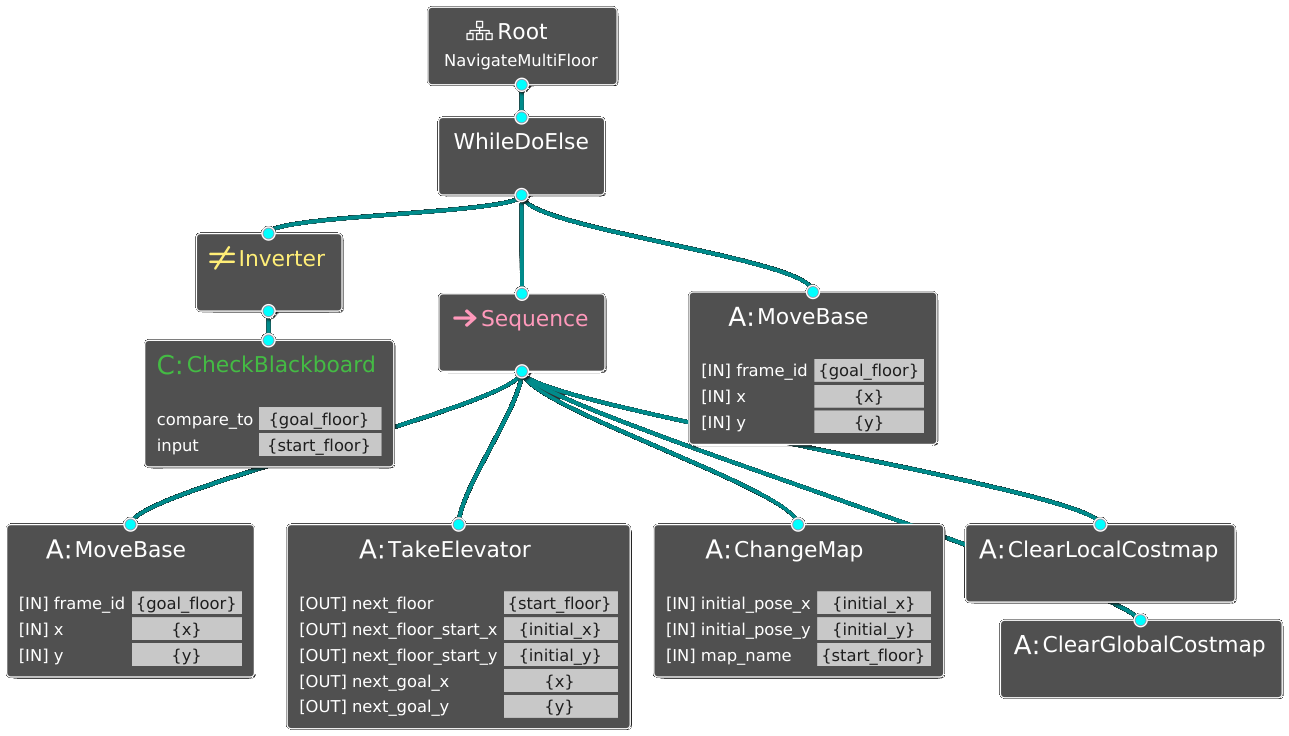
\includegraphics[width=\textwidth]{figures/50_implementation/bt_navigate_multi_floor.png}
    \caption[BT of the multi-floor navigation]{BT of the multi-floor navigation}
    \label{fig:bt_navigate_multi_floor}
\end{figure}

Figure \ref{fig:bt_navigate_multi_floor} shows the behavior of a single multi-floor navigation process. First, the left branch is checked as a break condition in the WhileDoElse control node. As long as the break condition is true, the middle branch is executed; if it is false, the right branch is executed and the while loop is terminated, along with the entire tree. The condition checks if the current floor value stored in the \texttt{start\_floor} variable is the same as the \texttt{goal\_floor}. The result of this check is then inverted and used as the break condition of the while loop. This means that as long as the floors are different, the middle branch is executed, and when the robot reaches the same floor as the goal floor, the right branch is executed only once. The sequence in the middle triggers all its children from left to right and performs a full floor change. Starting with the MoveBase action, which calls the action interface of the \gls{nav_2} stack. This uses the \texttt{goal\_floor} as \texttt{frame\_id} as described in the section above. The x and y coordinates of the goal for this action also describe the position of the goal on the goal floor. Note that the custom planner plugin always returns only the part of the path that is on the current floor. Since the hierarchical path of the H-Graph knows which elevator to take to reach the goal floor in the shortest distance, it will determine the position that is returned to the \gls{nav_2} stack and executed by the robot. After the MoveBase action, the robot stands in front of the elevator. The next step is to trigger the necessary actions to perform this elevator transport. As discussed earlier, in simulation this is just a teleport and for the PeTRA use case this will be a complete subtree coordinating the movement of the arm to press the right buttons inside the elevator. The output of this action is the next floor the robot has to go to, the initial position on the map of this new floor, and the goal position on this floor. Depending on the hierarchical path, this can be the final goal or another elevator position, which causes the WhileDoElse to loop again. Next the map has to be changed and the initial pose of the robot has to be set. Before planning on this new map, the cached local and global costmaps of the old floor must be cleared. Once this is done, the condition is evaluated again and either another map change is performed or the last floor is reached and the MoveBase to the last goal pose is executed. When this goal pose is reached, the loop is exited and the behavior tree is successfully finished.